\chapter{Communication Systems - Part II}\label{chap10}

\vskip -.25cm

The fundamental purpose of an electronic communication system is to transfer information from one place to another. Electronic communication involves the transmission, reception and processing of information between two or more locations using electronic circuits. In the early days hand gestures, facial expression, verbal grunts and groans were used for short distance communications and for long distance communications smoke signals or tom-tom drums were used.

Long distance communication using electricity began in 1837, when Morse invented the first workable telegraph. In 1876, Alexander Graham Bell and Thomas A. Watson successfully transmitted human conversation over a crude metallic wire communication system using the telephone.

With parallel advances in IC technology, computer science, signal processing, communication techniques, {\em today} we have very sophisticated communication systems to transfer speech, text, video over larger distances at an unimaginable speed.

This chapter begins with basic terminologies used in communication system and the operation of telephone system. Other communication systems such as mobile communication system, ISDN and optical fibre communication systems have also been discussed.

\vskip -1.2cm

\section{Basic terminologies and their definitions}\label{sec10.1}

Some basic terminologies\index{Communication systems!basic terminologies} and their definitions are given below, which are helpful in under standing the operation of different communication systems.

\vskip -1.2cm

\subsection{Data transmission modes in communication circuits}\label{sec10.1.1}

\heading{Simplex}
\smallskip

In the simplex mode, data transmission is unidirectional i.e., information can be sent in only one direction.

\vfill\eject

\heading{Half duplex}

\vskip .1cm

In the half-duplex mode, data transmission is possible in both directions but not at the same time.


\smallskip
\heading{Full duplex}
\vskip .1cm

In the full-duplex mode, transmissions are possible in both directions simultaneously, but they must be between the same two stations.

\smallskip
\heading{Full/Full duplex}
\vskip .1cm

In the full/full duplex mode, transmission is possible in both directions at the same time but not between the same two stations.

\subsection{Telephone system}\label{sec10.1.2}
\index{Telephone system}

\heading{Instrument, Station and Subscriber}
\vskip .1cm

An instrument is any device used to originate and terminate calls and to transmit and receive signals into and out of the telephone network. The place where the instrument is located is called the station.

The operator or user of the instrument is called the subscriber.


\smallskip
\heading{Local loops}
\vskip .1cm

The local loop is the dedicated cable facility used to connect an instrument at subscriber's station to the nearest telephone office.

\smallskip
\heading{Trunk circuits}
\vskip .1cm

Trunk circuits are used to interconnect two telephone offices.

\smallskip
\heading{Transceiver} 
\vskip .1cm

A device comprising both a transmitter and a receiver which are combined and share the same circuits. 

\smallskip
\heading{Public switching telephone network (PSTN)}
\vskip .1cm

PSTN is the aggregate of the worlds circuit switched telephone network that are operated by national, regional or local telephony operators providing infrastructure and services for public telecommunication. The PSTN consists of telephone lines, Fibre optic cables, microwave transmission links, cellular network, communication satellites and under sea telephone cables.

\smallskip
\heading{Modem}\index{Modem}
\vskip .1cm

A modem ({\em modulator-demodulator}) is a device that modulates signals to encode digital information during transmission and decode the received signal to reproduce the original digital data.

\section{The telephone systems}\label{sec10.2}
\index{Telephone systems}

\subsection{Introduction}\label{sec10.2.1}

The word telephone comes from the Greek words tele meaning ``from far'' and phone, meaning ``sound'', ``voice'' or ``voiced sound''.

To talk to some one, we simply pickup the phone and dial a few digits, and we are almost instantly connected to them.

Telephone systems were originally developed for conveying human speech information. Nowadays, with the use of modems, telephone systems are also extensively used to transport data, fascimile and even video.

Any one who uses a telephone or a data modem on a telephone circuit, is a part of global communication network called PSTN. The PSTN uses the largest computer network in the world to inter connect millions of subscribers. 

The telephone is one of the simplest devices ever developed, and the telephone connection has not changed in nearly a century, inspite of advances like fibre optics and digital signal transmission. 

A simple dial type telephone can be connected with modern data communication equipment with minor changes (some times even without), since the compatibility is maintained in most areas of the system.

\subsection{Working of telephone system}\label{sec10.2.2}
\index{Telephone systems!working of}

The basic topology of\index{Telephone systems!topology of} a typical switched telephone system is shown in Fig.~\ref{fig10.1}.
\begin{figure}[H]
\centering
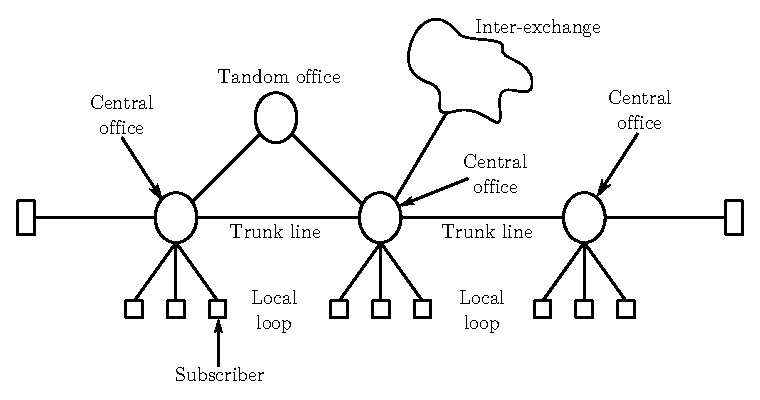
\includegraphics[scale=.94]{chap10/fig10.1.eps}
\caption{Typical telephone network}\label{fig10.1}
\end{figure}
\begin{itemize}
\item[$\bullet$] Each subscriber of the telephone system is connected to a central office. The central office represents an exchange, which is a central location where subscribers are interconnected.

\item[$\bullet$] Subscribers connected to the same central office can communicate with each other by means of central office switch which can connect any line to any other line.

\item[$\bullet$] The central offices are connected together by trunk line. This establishes the inter connection between customers from different central offices.

\item[$\bullet$] In larger metropolitan areas it is virtually impossible to provide trunk connection between all the central offices. In such cases tandom offices are used to establish the connection.

\item[$\bullet$] Each individual subscriber telephone is connected to the central office by single twisted pair of wires. Twisting of wires help to cancel the crosstalk. Cross talk is a disturbance created in the communication line, when two metalic conductors carrying different signals are located close to each other.

\item[$\bullet$] Two types of dialing systems are employed:
\begin{itemize}
\item[(a)] Rotary dialing

\item[(b)] Dual Tone Multi-Frequency (DTMF) dialing
\end{itemize}
\end{itemize}

Rotary dialing is an old method of dialing. It functions by breaking the loop circuit at 10\,Hz rate, with the number of interruptions equal to the number dialed. It is also called pulse dialing.

In DTMF, a combination of two tones is transmitted for each number. It is also called as touch tone dialing.

\subsection{Telephone set (Telephone instrument)}\label{sec10.2.3}
\index{Telephone set}

Fig.~\ref{fig10.2} shows the functional block diagram of a standard telephone set.

It consists of the following components.
\begin{itemize}
\item[(a)] Ringer circuit

\item[(b)] On/of hook circuit

\item[(c)] Equalizer circuit

\item[(d)] Speaker

\item[(e)] Microphone

\item[(f)] Hybrid network

\item[(g)] Dialing circuit
\end{itemize}

\begin{figure}[H]
\centering
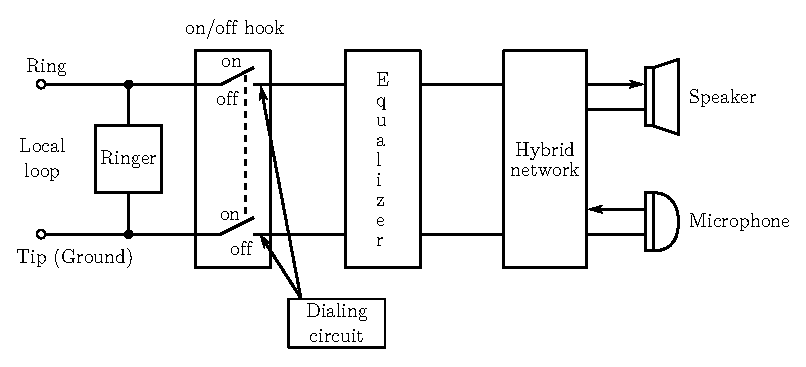
\includegraphics[scale=.9]{chap10/fig10.2.eps}
\caption{Functional block diagram of a Telephone set}\label{fig10.2}
\end{figure}
\begin{itemize}
\item[$\bullet$]
The purpose of the ringer is to alert the destination party of incoming calls. In the early telephones the ringer circuit was an electromagnetic bell placed directly across the local loop. In modern telephones, the bell has been replaced by an electronic oscillator connected to the speaker.

\item[$\bullet$]
The on/off hook circuit is an STDP (single throw double pole) switch which is mechanically connected to the handset. The switch is open when the telephone is idle. When the telephone is in use, the switch is closed completing the electrical path through the microphone between the tip and ring of the local loop.

\item[$\bullet$]
Equalizer circuit is used to regulate the amplitude and frequency response of the voice signals. It comprises of resistors, inductors and capacitors.

\item[$\bullet$]
Speaker is the receiver for the telephone. It converts electrical signals received from the local loop to sound waves that can be heard and {\em under stood} by the listener. 

\item[$\bullet$]
The microphone is the transmitter for the telephone, which converts accoustical signals in the form of sound pressure waves from the caller to electrical signals that are transmitted into the telephone network through the local subscriber loop.

\item[$\bullet$]
The local loop is a two wire circuit and the telephone set is a four wire circuit; two for transmitter and two for receiver. The hybrid network converts a two wire circuit into a four wire circuit.

\item[$\bullet$]
The dialing circuit enables the subscriber to output signals representing digits, and this enables the caller to enter the destination telephone number.
\end{itemize}

\section{Mobile Telephone (Cellular Telephone)}\label{sec10.3}

Cellular telephone\index{Cellular telephone} offers full-duplex transmissions and operates much the same way as the standard wire line telephone services provided to homes and offices by local telephone companies. Mobile telephone\index{Mobile telephone} system is a one to one system that permits two way simultaneous transmissions. Each cellular phone is assigned a unique telephone number for privacy. 

In a conventional communication system a single transmitter and receiver are used to cover a wide geographical area. With the cellular concept, each area is further divided into hexagon - shaped cells that fit together to form a honey comb pattern as shown in Fig.~\ref{fig10.3}.
\begin{figure}[H]
\centering

\includegraphics{chap10/fig10.3.eps}
\caption{Division of geographical area into hexagonal cells}\label{fig10.3}
\end{figure}

The reason for chosing hexagon shape is two fold.
\begin{itemize}
\item[$\bullet$] It provides the most effective transmission by approximating a circular pattern.

\item[$\bullet$] It eliminates the gaps present between adjacent circles.
\end{itemize}

Each cell is equipped with its own receiver and low power transmitter and covers several square kilometers of area.

Fig.~\ref{fig10.4} shows a simplified cellular telephone system.

It consists of the following components.
\begin{itemize}
\item[(a)] Mobile stations or mobile units

\item[(b)] Base stations

\item[(c)] Mobile telephone switching office (MTSO)
\end{itemize}

Each mobile station\index{Mobile station} consists of a transceiver, and antenna and control unit. The mobile unit may be inside an automobile or with a pedestrian.
\begin{figure}[H]
\centering
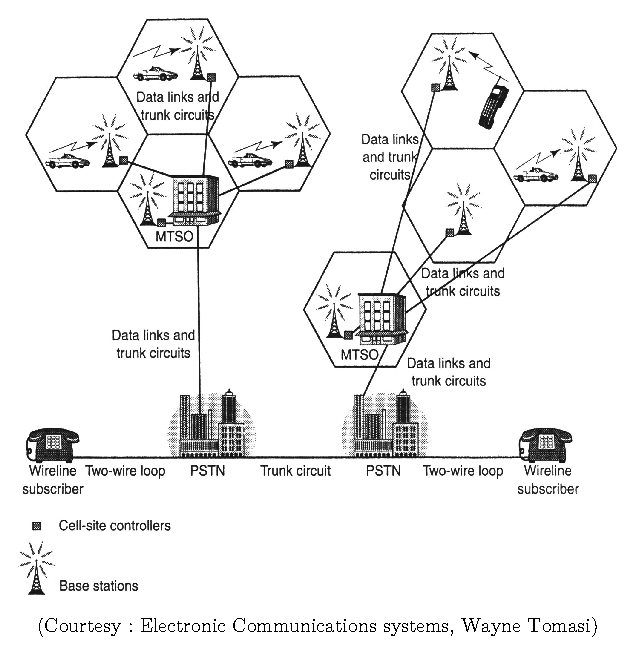
\includegraphics[scale=.92]{chap10/fig10.4.eps}
\caption{Simplified cellular telephone system}\label{fig10.4}
\end{figure}

Base stations\index{Base stations} are radio frequency tranceivers located within each cell. A base station serves as central control unit for all users with in that cell.

Base stations are distributed over the area of system coverage and are managed and controlled by an on-site computerised cell-site controller. The presence of base stations with in each cell enhances the transmission quality.

Base station consists of several transmitters and receivers which simultaneously handle full-duplex communication and generally have towers which support several transmitting and receiving antennas.

The function of the base station is to provide an interface between mobile telephone units and the MTSO. It connects the simultaneous mobile calls via telephone lines or microwave link to the MTSO. The MTSO provides a centralised administration and maintenance point for the entire network.

Today almost all cellular telephone systems provide roaming service. Roaming is when a mobile unit moves from one cell to another, possibly from one company's service area into another company's service area. The roaming facility is provided to user through a process called hand off in which a mobile unit is handed over from one base station's control to another base station's control. The MTSO is also called the mobile switching centre (MSC). An MTSO controls channel assignment, call processing, call setup and call termination.

The cellular system operates in the frequency range of 800-900 \,MHz range. Advanced cellular systems employ digital transmission and operate with a much greater capacity. These systems operate in 1.7-1.8\,GHz bands.

\subsection{Mobile telephone unit (Cellular Telephone Unit)}\label{sec10.3.1}

Mobile telephone unit is a portable telephone unit which receives or make calls through a base station or transmitting tower. Radio waves are used to transmit signals to and from the cell phone.

Fig.~\ref{fig10.5} shows the block diagrams of a cellular mobile unit. It consists of the following blocks.
\begin{center}
\begin{tabular}{r@{\;\,}l@{\qquad\qquad}r@{\;\,}l@{\qquad\qquad}r@{\;\,}l}
1. & Control unit & 2. & Logic unit & 3. & Receiver\\[4pt]
4. & Frequency synthesizer & 5. & Transmitter
\end{tabular}
\end{center}
\begin{figure}[H]
\centering
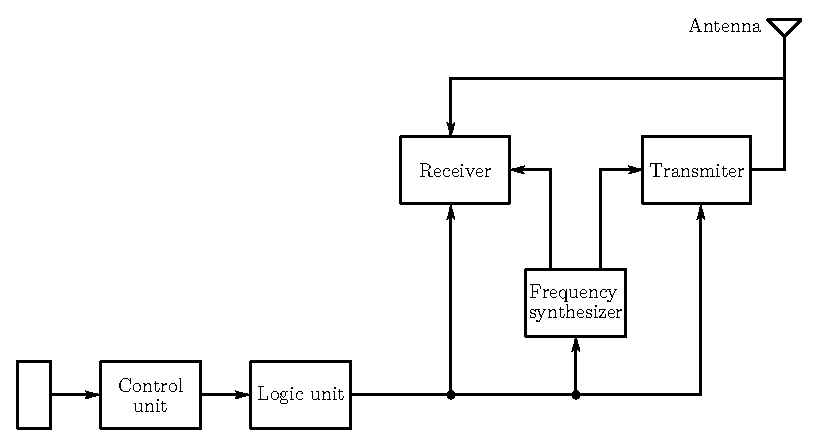
\includegraphics{chap10/fig10.5.eps}
\caption{Block diagram of mobile Telephone unit}\label{fig10.5}
\end{figure}

\section{Integrated Services Digital Network (ISDN)}\label{sec10.4}

The Integrated Services Digital Network (ISDN)\index{Integrated Services Digital Network (ISDN)} is a proposed network designed by the major telephone companies in conjunction with the ITU-T with the intent of providing world wide telecommunications support of voice, data, video, and fascimile information with in the same network.

ISDN is the integrating of a wide range of services into a single multipurpose network. ISDN is a network that proposes to interconnect an unlimited number of independent users through a common communication network.

To date, only a small number of ISDN facilities have been developed. How ever the telephone industry is presently implementing an ISDN system so that in the near future, subscribers will access the ISDN system using existing public telephone and data network.

Fig.~\ref{fig10.6} shows the subscribers conceptual view of ISDN.
\begin{figure}[H]
\centering
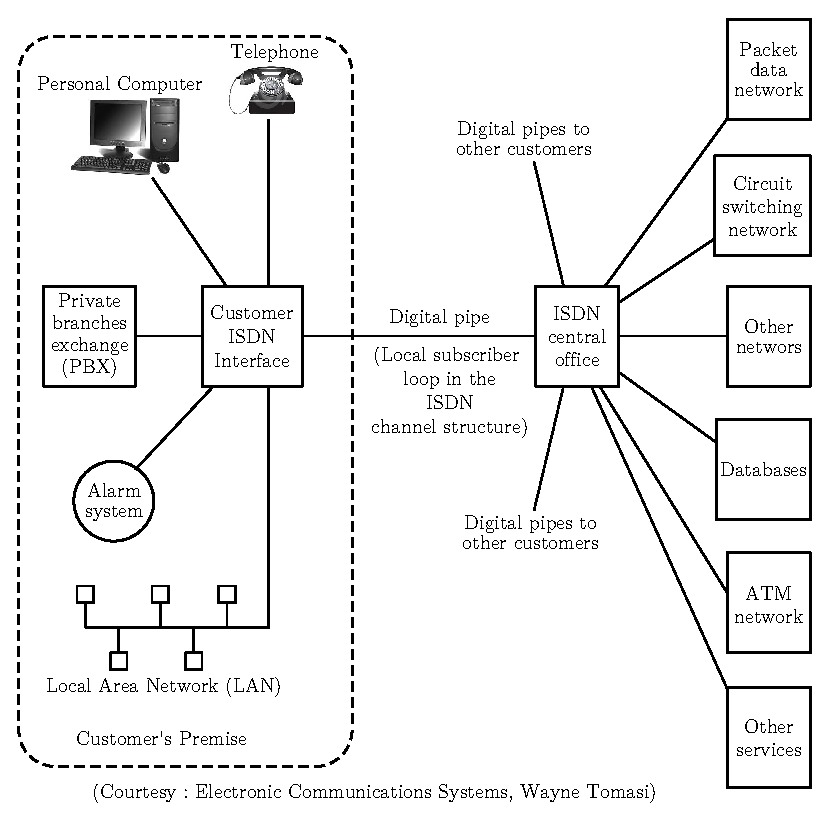
\includegraphics[scale=.8]{chap10/fig10.6.eps}
\caption{Conceptual view of ISDN}\label{fig10.6}
\end{figure}
\begin{itemize}
\item[$\bullet$] Customers gain access to the ISDN system through a local interface connected to a digital transmission medium called a digital pipe.

\item[$\bullet$] Depending upon the customer need, several sizes of pipe are available with varying capacities (i.e., bit rates).

\item[$\bullet$] A residential customer may require only enough capacity to accommodate a telephone and a personal computer.

\item[$\bullet$] An office complex may require a pipe with sufficient capacity to handle a large number of digital telephones interconnected through an on-premise private branch exchange (PBX) or a large number of computers on a local area network (LAN).
\end{itemize}
There are three basic types of ISDN channels.
\begin{enumerate}
\item Bearer (B) channel

\item Data (D) channel

\item Hybrid (H) channel
\end{enumerate}

B channel operates at 64\,kbps.

\vskip .1cm

D channel operates either at 16 or 64\,kbps depending upon the users need.

\vskip .1cm

H channels are available with data rates of 384\,kbps, 1536\,kbps or 1920\,kbps. These high data rates are suitable for applications such as video, teleconferencing and many other digital techniques. 

\section{Optical Fibre Communication System}\label{sec10.5}
\index{Communication systems!optical fibre}

Optical fibre\index{Optical fibre} cables are the newest and probably the most promising type of guided transmission medium for virtually all forms of digital data communication applications, including local, metropolitan, and wide area network. An optical fibre is made up of transparent material. Electromagnetic light waves are guided through this transparent media, without using electrical current flow.

An optical communication system\index{Optical communication system} uses the light as the carrier of information. Since it is difficult and often impractical to propagate light waves through earth's atmosphere, optical fibre communication systems use glass or plastic fibre cables to guide and transmit light waves. The optical fibre cables guide light waves in a manner similar to the way electromagnetic waves guided through a metallic transmission media.

\subsection{Block diagram of an optical fibre communication system}\label{sec10.5.1}

Fig.~\ref{fig10.7} shows a simplified block diagram of\index{Optical communication system!block diagram of} a simplex optical fibre communication system. The main building blocks are as follows.
\begin{enumerate}
\item The transmitter

\item The optical fibre cable

\item The receiver
\end{enumerate}
\begin{figure}[H]
\centering
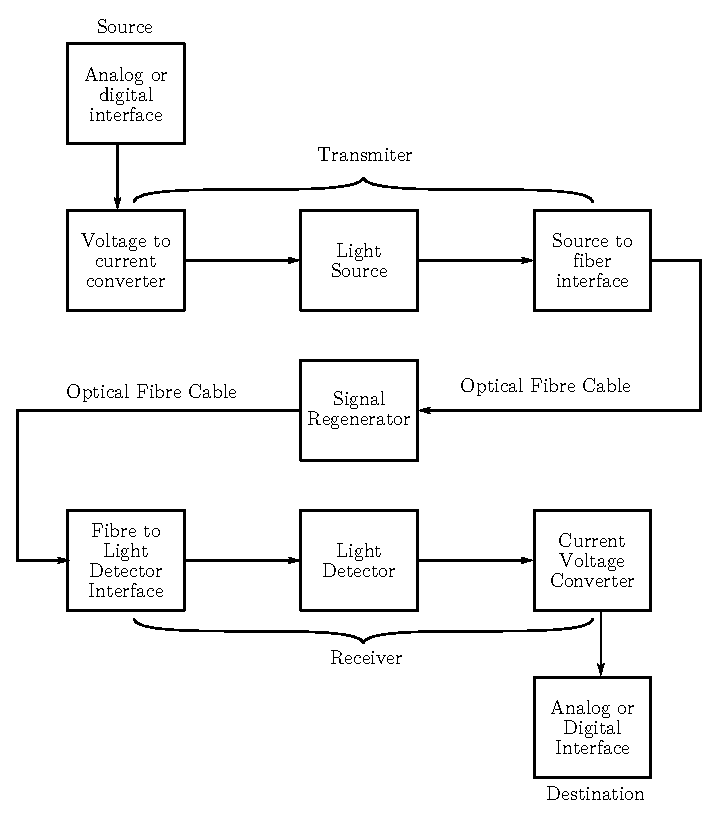
\includegraphics{chap10/fig10.7.eps}
\caption{Optical fibre communication system}\label{fig10.7}
\end{figure}

The source generates the information to be transmitted which may be either in analog or digital form. The source is interfaced with the transmitter through the analog or digital interface.

The analog or digital interface is an electrical interface that is used to match the impedance and signal level between the information source and the transmitter input.

The transmitter consists of the following blocks.
\begin{itemize}
\item[(a)] Voltage-to-current (V-I) converter

\item[(b)] Light source and

\item[(c)] Source to fibre interface
\end{itemize}

The {\em Voltage-to-current converter} converts an input signal voltage to a current. This current is used to drive the light source.

The {\em light source} is either an intrared  light emitting diode (LED) or an injection laser diode (ILD). The amount of light emitted by the light source is directly proportional to the current output from the V-I converter.

The function at the source can be summarised as follows.
\begin{itemize}
\item[$\bullet$] V-I converter converts the input signal voltage to a current and this current drives the light source.

\item The light source produces the light whose intensity is directly proportional to the current output of V-I converter (which inturn is directly proportional to the magnitude of source voltage)
\end{itemize}
$\Rightarrow$~ {\em Light intensity modulated by the source signal.}

The source-to-fibre coupler is an optical lens that couples the light emitted by the light source into the optical fibre cable.

The optical fibre consists of a glass or plastic fibre core surrounded by a cladding and encapsulated in a protective jacket.

The signal regenerator performs light amplification. In reality the signal is not actually amplified but it is reconstructed. If the distance between transmitter and receiver is too long, more regenerators are required.

The receiver consists of the following blocks.
\begin{itemize}
\item[(a)] Fibre to light detector interface

\item[(b)] Light detector

\item[(c)] Current to voltage converter
\end{itemize}

\eject

The light detector converts light energy to current. The following devices are generally used as light detectors.
\begin{itemize}
\item[(i)] PIN ($p$-type-intrinsic-$n$-type) device 

\item[(ii)] APD (avalanche photo diode)

\item[(iii)] Photo transistor
\end{itemize}

The current to voltage converter transforms changes in detector current to changes in voltage.

The analog or digital interface is used to match the impedance and signal level between the receiver output and the destination.

\subsection{Advantages of optical fibre cables}\label{sec10.5.2}
\index{Optical communication system!advantages of}

Following are the advantages of using optical fibres.

\smallskip
\heading{1. Wider bandwidth and greater information capacity}

\vskip .1cm
Optical fibres have greater information capacity than metallic cables because of the inherently wider bandwidths available with optical frequencies. Modern optical fibre communication systems are capable of transmitting several gigabytes per second over hundreds of kilometres. Hence a large number of individual voice and data channels can be combined and transmitted over one optical fibre cable.

\smallskip
\heading{2. Large distance transmission}

\vskip .1cm
Optical fibres have considerably less signal loss than metallic cables. Hence data can be transmitted over longer distances with less number of optical regenerators and amplifiers.

\smallskip
\heading{3. Enhanced signal security}

\vskip .1cm
Optical fibre cables are more secure than metallic cables. It is highly impossible to tap information from optical fibre cable and optical cables cannot be detected with metal detectors.

\smallskip
\heading{4. Durable and reliable}

\vskip .1cm
Optical fibre cables have a high degree of tolerance to changes in environmental conditions and are more immune to corrosive materials. Hence optical fibre cables last longer and more reliable than metallic conductors.

\smallskip
\heading{5. Immunity to cross talk}

\vskip .1cm
Optical fibres are made of glass and plastic fibres, which are non conductors of electrical current. Hence they are not surrounded by a changing magnetic field which is the primary source of cross talk in closely placed metallic cables. Hence optical fibre cables are immune to cross talk.

\eject

\heading{6. Immunity to electrical interference}

\vskip .1cm
Since optical fibre cables are non conductors of electrical current they are immune to electromagnetic interference (EMI) caused by lightning, electric motors, relays, fluorescent lights and other electrical noise sources.

\smallskip
\heading{7. Safety and convenience}

\vskip .1cm
Since optical fibres are non conductors, there are no electrical currents or voltage associated with them. Hence optical fiber cables are safer, easier to install and maintain than metallic cables.

Due to their small size, light weight and compactness than metallic cables, optical fibre cables are more flexible, easier to work with, requires less space for storage and cheaper to transport.

\smallskip
\heading{8. Economy}

Although the cost of optical fibre cable is approximately the same as metallic cables, less number repeaters are required due to low loss. This greatly reduces the installation and overall system costs.

\subsection{Applications of optical fibre communication}\label{sec10.5.4}
\index{Optical communication system!applications of}

Optical fibre cables find numerous applications owing to their advantages given above. Some of the important applications are as follows.
\begin{enumerate}
\item Optical fibre communication is preformed for all public network applications since OFC system is more efficient and economical.

\item Since optical fibres are non conductors of electricity, optical fibre cables can be used under the sea with enhanced electrical safety.

\item Optical fibre communication is extensively used in public service organisations such as railways, TV transmissions etc.

\item Educational institutions, universities, offices, industries, business organisations etc. employ optical fibres with in their LAN (Local Area Network) systems.

\item Optical fibre communication is widely used in telecommunication. These applications include voice telephones, video phones, telegraph services, message services etc.
\end{enumerate}


\begin{thebibliography}{99}
\bibitem{key1} David A. Bell, Electronic Devices and Circuits, 5e, Oxford University press, India, 2009.

\bibitem{key2} D. P. Kothari, I. J. Nagarath, Basic Electronics, Mc Graw Hill Education (India) Private Limited, 2014.

\bibitem{key3} Ramesh S. Gaonkar, Microprocessor Architechture, Programming and Applications, 3e, Penram International Publishing, India, 1997.

\bibitem{key4} Ayala, The 8051 Microcontroller, 3e, Thomson Learning Inc., 2007.

\bibitem{key5} Dr. K. Uma Rao and Dr. Andhe Pallavi, The 8051 Microcontroller Architecture, Programming and Applications, Sanguine Technical Publishers, India, 2009.

\bibitem{key6} V. Udayashankara and M. S. Mallikarjuna Swamy, 1e Tata Mc Graw Hill Publishing Company Limited, India, 2009.

\bibitem{key7} Wayne Tomasi, Electronic Communications Systems, 5e, Pearson Education, 2011.

\bibitem{key8} Deobelin and Manik, Measurement Systems, 6e Mc Graw Hill Education (India) Private Limited, 2013.

\bibitem{key9} B. Somanathan Nair, Deepa S. R., Electronic Instrumentation, Sanguine Technical Publishers, India, 2008.
\end{thebibliography}
